\documentclass{article}

\usepackage{graphicx}
\usepackage{tikz}
\usepackage{tikzsymbols}
\usetikzlibrary{calc,patterns,shapes.geometric}
\pagestyle{empty}
\usepackage[margin=0pt]{geometry}
\geometry{papersize={14in,12in}}

\def\centerarc[#1](#2)(#3:#4:#5){\draw[#1] ($(#2)+({#5*cos(#3)},{#5*sin(#3)})$) arc (#3:#4:#5);}

\begin{document}
	\begin{figure}
		\centering
		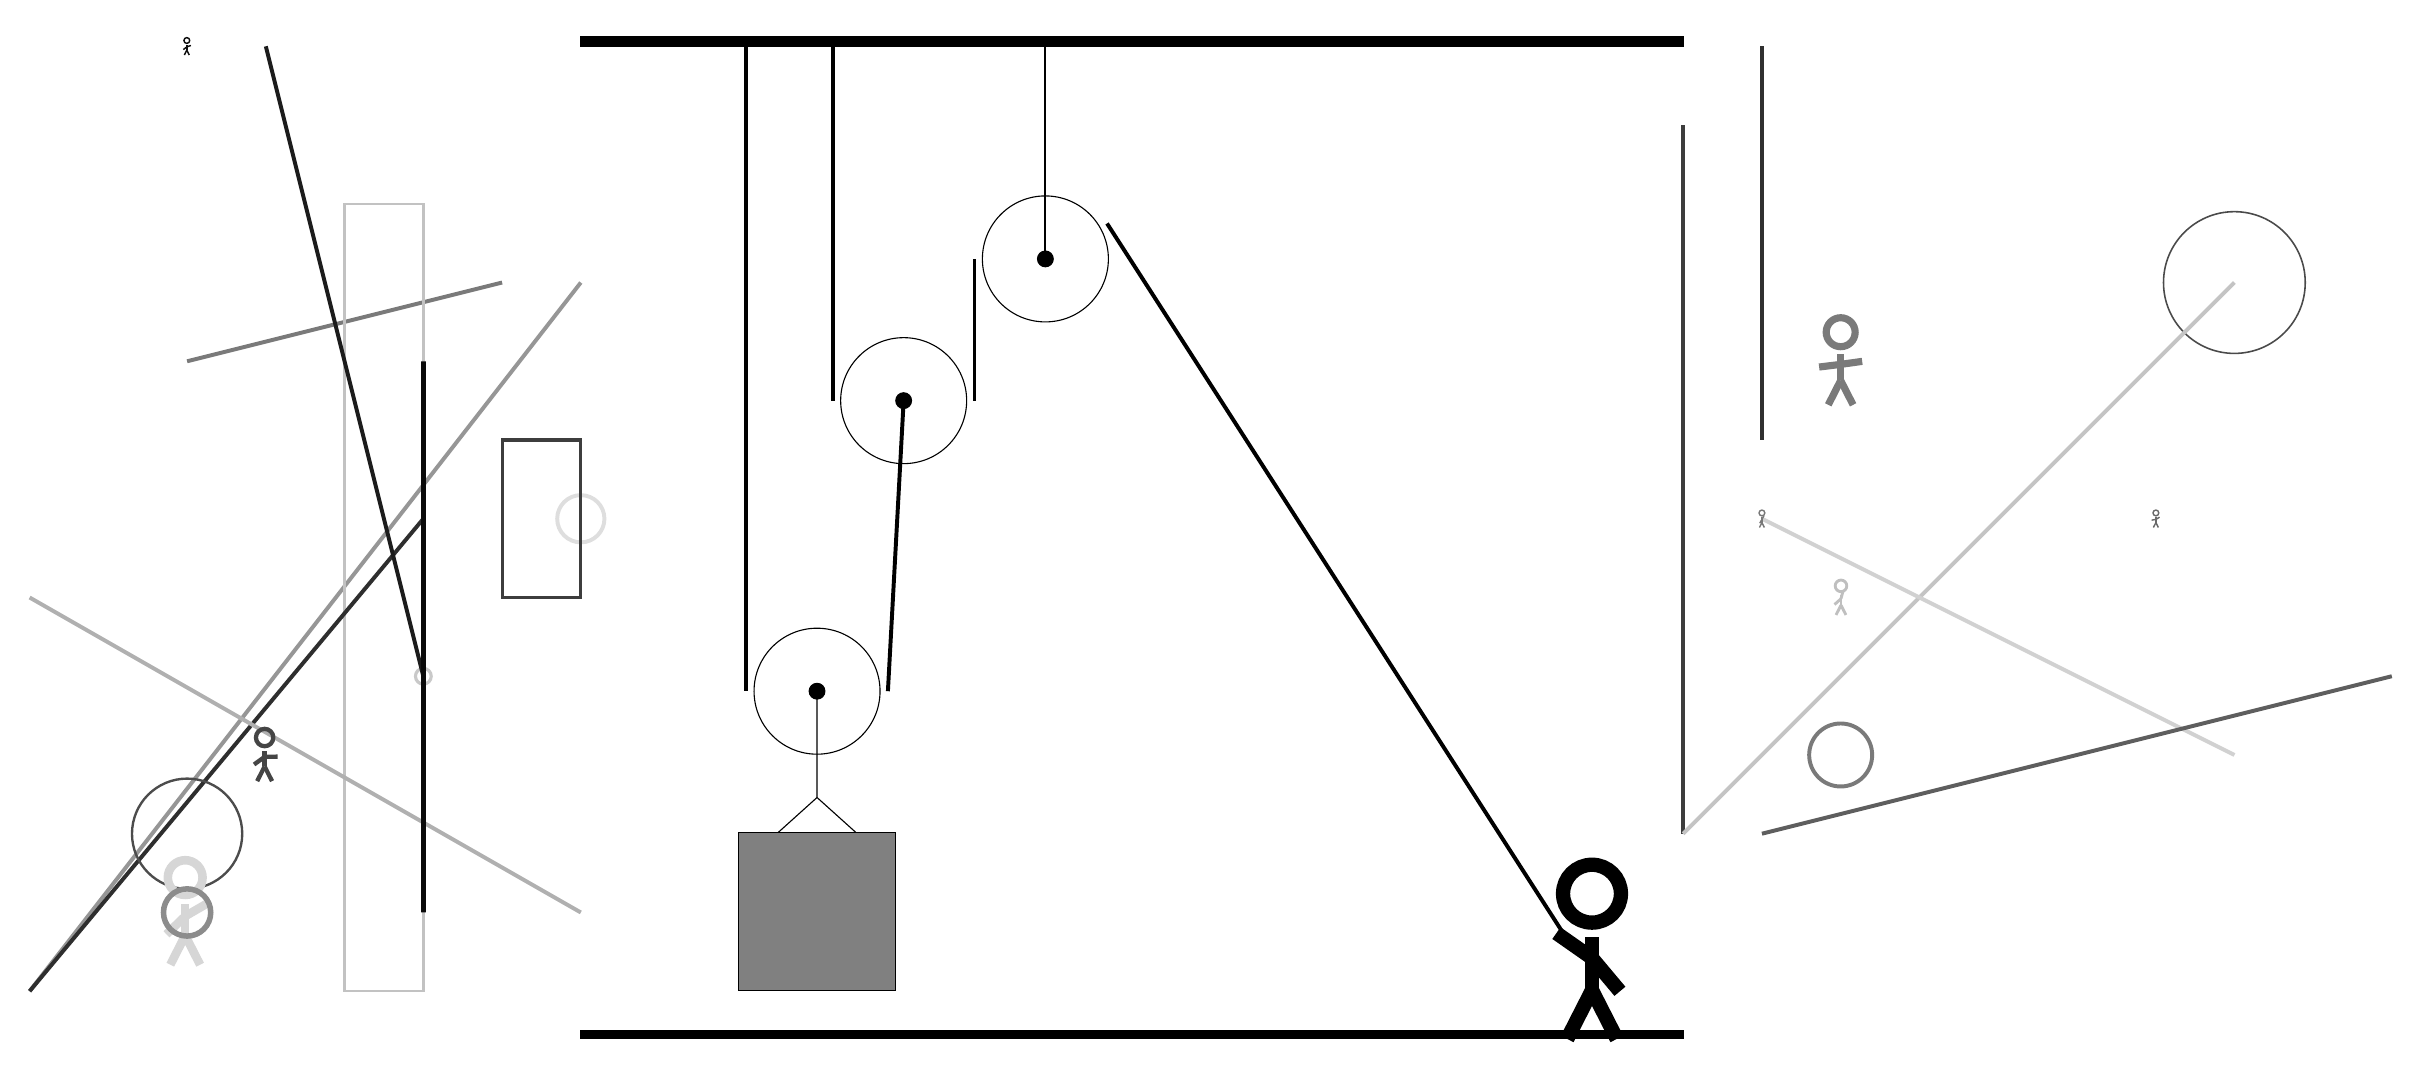
\begin{tikzpicture}
			%%%%% START %%%%%
			
			\draw[fill=black] (-2, 9) rectangle (12, 9.125);
			
			\draw (1, 0.81) circle (0.8);
			\draw[fill=black] (1, 0.81) circle (0.1);
			
			\draw (2.1, 4.5) circle (0.8);
			\draw[fill=black] (2.1, 4.5) circle (0.1);
			
			\draw (3.9, 6.3) circle (0.8);
			\draw[fill=black] (3.9, 6.3) circle (0.1);
			\draw[thick] (3.9, 6.3) -- (3.9, 9);
			
			\draw (1, 0.81) -- (1, -0.54) -- (0.5, -0.99) -- (1.5, -0.99) -- (1, -0.54);
			\draw[fill=black!50] (0, -0.99) rectangle (2, -2.99);
			
			\draw[line width=0.5mm] (0.1, 9) -- (0.1, 0.81);
			\centerarc[line width=0.5mm](1, 0.81)(180:360:0.9);
			\draw[line width=0.5mm](1.9, 0.81) -- (2.1, 4.5);
			\draw[line width=0.5mm] (1.2, 9) -- (1.2, 4.5);
			\centerarc[line width=0.5mm](2.1, 4.5)(180:360:0.9);
			\draw[line width=0.5mm](3.0, 4.5) -- (3.0, 6.3);
			\centerarc[line width=0.5mm](3.9, 6.3)(30:180:0.9);
			\draw[line width=0.5mm] (4.683, 6.75) -- (10.5, -2.3);
			
			\node at (10.8, -2.5) {\Strichmaxerl[10][-35][-50]};
			
			\draw[line width=0.5mm, color=black!52](-3, 6) -- (-7, 5);
			
			\draw[line width=0.5mm, color=black!41](-2, 6) -- (-9, -3);
			\draw [line width=0.4mm, color=black!21](-4, 1) circle (0.1);
			\draw[line width=0.3mm, color=black!24] (-4, 7) rectangle (-5, -3);
			\draw[line width=0.5mm, color=black!82](-4, 3) -- (-9, -3);
			\draw[line width=0.5mm, color=black!31](-2, -2) -- (-9, 2);
			\draw [line width=0.3mm, color=black!70](-7, -1) circle (0.7);
			\draw [line width=0.2mm, color=black!71](19, 6) circle (0.9);
			\draw [line width=0.5mm, color=black!13](-2, 3) circle (0.3);
			\draw[line width=0.5mm, color=black!76](12, -1) -- (12, 8);
			
			\node[line width=0.2mm, color=black!16] at (-7, -2) {\Strichmaxerl[6][44][30]};
			\draw [line width=0.7mm, color=black!45](-7, -2) circle (0.3);
			\draw[line width=0.5mm, color=black!89](-6, 9) -- (-4, 1);
			
			\node[line width=0.5mm, color=black!52] at (14, 5) {\Strichmaxerl[5][7][8]};
			\node[line width=0.3mm, color=black!73] at (-6, 0) {\Strichmaxerl[3][36][1]};
			\draw [line width=0.5mm, color=black!52](14, 0) circle (0.4);
			
			\draw[line width=0.5mm, color=black!23](12, -1) -- (19, 6);
			
			\draw[line width=0.5mm, color=black!18](13, 3) -- (19, 0);
			\draw[line width=0.4mm, color=black!76] (-2, 4) rectangle (-3, 2);
			\node[line width=0.3mm, color=black!53] at (13, 3) {\Strichmaxerl[1][61][61]};
			\node[line width=0.7mm, color=black!59] at (18, 3) {\Strichmaxerl[1][10][31]};
			\draw[line width=0.6mm, color=black!96] (-4, -2) rectangle (-4, 5);
			\node[line width=0.7mm, color=black!25] at (14, 2) {\Strichmaxerl[2][42][75]};
			\node[line width=0.3mm, color=black!95] at (-7, 9) {\Strichmaxerl[1][37][20]};
			\draw[line width=0.5mm, color=black!81](13, 9) -- (13, 4);
			
			\draw[line width=0.5mm, color=black!63](13, -1) -- (21, 1);
			
			\draw[fill=black] (-2, -3.5) rectangle (12, -3.6);
			
			%%%%% END %%%%%
		\end{tikzpicture}
	\end{figure}	
\end{document}